\clearpage
\subsubsectionold{MSVC + \olly}
\myindex{\olly}

Let's load our example into \olly 
and see, what values are set in EAX/EBX/ECX/EDX after the execution of CPUID: 

\begin{figure}[H]
\centering
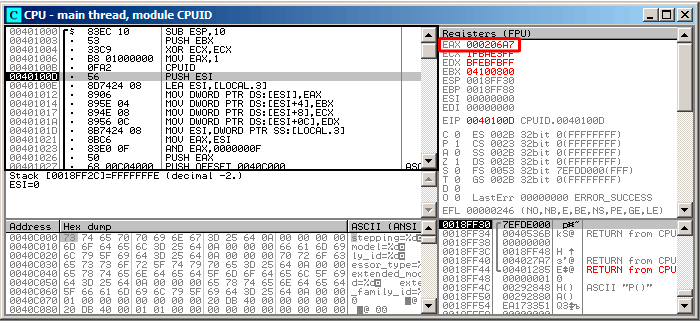
\includegraphics[scale=\FigScale]{patterns/15_structs/6_bitfields/cpuid/olly.png}
\caption{\olly: After CPUID execution}
\label{fig:cpuid_olly_1}
\end{figure}

EAX has \TT{0x000206A7} (my \ac{CPU} is Intel Xeon E3-1220).\\
This is $0000 0000 0000 0010 0000 0110 1010 0111$ in binary form.

Here is how the bits are distributed by fields:

\begin{center}
\begin{tabular}{ | l | l | l | }
\hline
\headercolor{} field &
\headercolor{} in binary form &
\headercolor{} in decimal form \\
\hline
reserved2		& 0000 & 0 \\
\hline
extended\_family\_id	& 00000000 & 0 \\
\hline
extended\_model\_id	& 0010 & 2 \\
\hline
reserved1		& 00 & 0 \\
\hline
processor\_id		& 00 & 0 \\
\hline
family\_id		& 0110 & 6 \\
\hline
model			& 1010 & 10 \\
\hline
stepping		& 0111 & 7 \\
\hline
\end{tabular}
\end{center}

\begin{figure}[H]
\centering
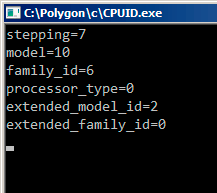
\includegraphics[scale=\NormalScale]{patterns/15_structs/6_bitfields/cpuid/result.png}
\caption{\olly: Result}
\label{fig:cpuid_olly_2}
\end{figure}
